\documentclass[12pt,twoside]{report}

%%%%%%%%%%%%%%%%%%%%%%%%%%%%%%%%%%%%%%%%%%%%%%%%%%%%%%%%%%%%%%%%%%%%%%%%%%%%%

% Definitions for the title page
% Edit these to provide the correct information
% e.g. \newcommand{\reportauthor}{Timothy Kimber}

\newcommand{\reporttitle}{Gap in Matematica e Fisica}
\newcommand{\reportauthor}{Luca Palumbo}
\newcommand{\reportclass}{V BSA}
\newcommand{\supervisor}{Name of supervisor}
\newcommand{\degreetype}{Type of Degree}

%%%%%%%%%%%%%%%%%%%%%%%%%%%%%%%%%%%%%%%%%%%%%%%%%%%%%%%%%%%%%%%%%%%%%%%%%%%%%

% load some definitions and default packages
%%%%%%%%%%%%%%%%%%%%%%%%%%%%%%%%%%%%%%%%%
% University Assignment Title Page 
% LaTeX Template
% Version 1.0 (27/12/12)
%
% This template has been downloaded from:
% http://www.LaTeXTemplates.com
%
% Original author:
% WikiBooks (http://en.wikibooks.org/wiki/LaTeX/Title_Creation)
%
% License:
% CC BY-NC-SA 3.0 (http://creativecommons.org/licenses/by-nc-sa/3.0/)
% 
%
%%%%%%%%%%%%%%%%%%%%%%%%%%%%%%%%%%%%%%%%%
%----------------------------------------------------------------------------------------
%	PACKAGES AND OTHER DOCUMENT CONFIGURATIONS
%----------------------------------------------------------------------------------------
\usepackage[a4paper,hmargin=2.8cm,vmargin=2.0cm,includeheadfoot]{geometry}
\usepackage{textpos}
\usepackage[square,numbers]{natbib} % for bibliography
\usepackage{tabularx,longtable,multirow,subfigure,caption}%hangcaption
\usepackage{fncylab} %formatting of labels
\usepackage{fancyhdr} % page layout
\usepackage{url} % URLs
%\usepackage[english]{babel}
\usepackage{amsmath}
\usepackage{graphicx}
\usepackage{dsfont}
\usepackage{epstopdf} % automatically replace .eps with .pdf in graphics
%\usepackage{backref} % needed for citations
\usepackage{array}
\usepackage{latexsym}
\usepackage[pdftex,pagebackref,hypertexnames=false,colorlinks]{hyperref} % provide links in pdf
% questi sono inseriti da Me
\usepackage[italian]{babel}
\usepackage{siunitx}
\usepackage{amsmath}
\usepackage{amsthm}
\usepackage[utf8]{inputenc}
\usepackage{listings}
\usepackage{xcolor}
\usepackage[nottoc]{tocbibind}
%\usepackage{cite}

%\usepackage{biblatex}


\hypersetup{pdftitle={},
  pdfsubject={}, 
  pdfauthor={},
  pdfkeywords={}, 
  pdfstartview=FitH,
  pdfpagemode={UseOutlines},% None, FullScreen, UseOutlines
  bookmarksnumbered=true, bookmarksopen=true, colorlinks,
    citecolor=black,%
    filecolor=black,%
    linkcolor=black,%
    urlcolor=black}

\usepackage[all]{hypcap}


%\usepackage{color}
%\usepackage[tight,ugly]{units}
%\usepackage{float}
%\usepackage{tcolorbox}
%\usepackage[colorinlistoftodos]{todonotes}
% \usepackage{ntheorem}
% \theoremstyle{break}
% \newtheorem{lemma}{Lemma}
% \newtheorem{theorem}{Theorem}
% \newtheorem{remark}{Remark}
% \newtheorem{definition}{Definition}
% \newtheorem{proof}{Proof}


%%% Default fonts
\renewcommand*{\rmdefault}{bch}
\renewcommand*{\ttdefault}{cmtt}



%%% Default settings (page layout)
\setlength{\parindent}{0em}  % indentation of paragraph

\setlength{\headheight}{14.5pt}
\pagestyle{fancy}
\renewcommand{\chaptermark}[1]{\markboth{\chaptername\ \thechapter.\ #1}{}} 

\fancyfoot[ER,OL]{\sffamily\textbf{\thepage}}%Page no. in the left on odd pages and on right on even pages
\fancyfoot[OC,EC]{\sffamily }
\renewcommand{\headrulewidth}{0.1pt}
\renewcommand{\footrulewidth}{0.1pt}
\captionsetup{margin=10pt,font=small,labelfont=bf}


%--- chapter heading

\def\@makechapterhead#1{%
  \vspace*{10\p@}%
  {\parindent \z@ \raggedright \sffamily
    \interlinepenalty\@M
    \Huge\bfseries \thechapter \space\space #1\par\nobreak
    \vskip 30\p@
  }}

%---chapter heading for \chapter*  
\def\@makeschapterhead#1{%
  \vspace*{10\p@}%
  {\parindent \z@ \raggedright
    \sffamily
    \interlinepenalty\@M
    \Huge \bfseries  #1\par\nobreak
    \vskip 30\p@
  }}

\allowdisplaybreaks

% load some macros
% Here, you can define your own macros. Some examples are given below.

\newcommand{\R}[0]{\mathds{R}} % real numbers
\newcommand{\Z}[0]{\mathds{Z}} % integers
\newcommand{\N}[0]{\mathds{N}} % natural numbers
\newcommand{\C}[0]{\mathds{C}} % complex numbers
\renewcommand{\vec}[1]{{\boldsymbol{{#1}}}} % vector
\newcommand{\mat}[1]{{\boldsymbol{{#1}}}} % matrix

% inseriti da me
\newtheorem{theorem}{Theorem}
\newtheorem{definition}{Definizione}
%\renewcommand{\chaptername}{Unità}
%\addto\captionsitalian{\renewcommand{\chaptername}{Sessione}}
%\renewcommand{\chapter}{Capitolo}




%New colors defined below
\definecolor{codegreen}{rgb}{0,0.6,0}
\definecolor{codegray}{rgb}{0.5,0.5,0.5}
\definecolor{codepurple}{rgb}{0.58,0,0.82}
\definecolor{backcolour}{rgb}{0.95,0.95,0.92}
\definecolor{dkgreen}{rgb}{0,0.6,0}
\definecolor{gray}{rgb}{0.5,0.5,0.5}
\definecolor{mauve}{rgb}{0.58,0,0.82}
%Code listing style named "mystyle"
\lstdefinestyle{mystyle}{
  backgroundcolor=\color{backcolour},   commentstyle=\color{codegreen},
  keywordstyle=\color{blue},
  numberstyle=\tiny\color{codegray},
  stringstyle=\color{codepurple},
  basicstyle=\ttfamily\footnotesize,
  breakatwhitespace=false,         
  breaklines=true,                 
  captionpos=b,                    
  keepspaces=true,                 
  numbers=left,                    
  numbersep=5pt,                  
  showspaces=false,                
  showstringspaces=false,
  showtabs=false,                  
  tabsize=2
}
\lstset{style=mystyle}

\date{Giugno 2021}

\begin{document}

% load title page
% Last modification: 2015-08-17 (Marc Deisenroth)
\begin{titlepage}

\newcommand{\HRule}{\rule{\linewidth}{0.5mm}} % Defines a new command for the horizontal lines, change thickness here


%----------------------------------------------------------------------------------------
%	LOGO SECTION
%----------------------------------------------------------------------------------------

\center 
\includegraphics[width = 4cm]{./figures/lorenzlogo}\\[0.1cm] 

\center % Center remainder of the page

%----------------------------------------------------------------------------------------
%	HEADING SECTIONS
%----------------------------------------------------------------------------------------

\textsc{\Large Liceo Statale ``C. Lorenzini''}\\[0.5cm] 
\textsc{\large Liceo Scientifico opzione Scienze Applicate}\\[0.5cm] 

%----------------------------------------------------------------------------------------
%	TITLE SECTION
%----------------------------------------------------------------------------------------

\HRule \\[0.4cm]
{ \huge \bfseries \reporttitle}\\ % Title of your document
\HRule \\[1.5cm]
 
%----------------------------------------------------------------------------------------
%	AUTHOR SECTION
%----------------------------------------------------------------------------------------

\begin{minipage}{0.4\textwidth}
%\begin{flushleft} \large
\center \emph{}\\
\reportauthor
%\end{flushleft}
\end{minipage}
~
%\begin{minipage}{0.4\textwidth}
%\begin{flushright} \large
%\emph{Supervisor:} \\
%\supervisor % Supervisor's Name
%\end{flushright}
%\end{minipage}\\[4cm]


%----------------------------------------------------------------------------------------
%	FOOTER & DATE SECTION
%----------------------------------------------------------------------------------------
\vfill % Fill the rest of the page with whitespace
%Submitted in partial fulfillment of the requirements for the MSc degree in
%\degreetype~of Imperial College London\\[0.5cm]

\makeatletter
\@date 
\makeatother


\end{titlepage}



% page numbering etc.
\pagenumbering{roman}
\clearpage{\pagestyle{empty}\cleardoublepage}
\setcounter{page}{1}
\pagestyle{fancy}

%%%%%%%%%%%%%%%%%%%%%%%%%%%%%%%%%%%%
%\begin{abstract}
%Your abstract.
%\end{abstract}

%\cleardoublepage
%%%%%%%%%%%%%%%%%%%%%%%%%%%%%%%%%%%%
%\section*{Acknowledgments}
%Comment this out if not needed.

%\clearpage{\pagestyle{empty}\cleardoublepage}

%%%%%%%%%%%%%%%%%%%%%%%%%%%%%%%%%%%%
%--- table of contents
\fancyhead[RE,LO]{\sffamily {Table of Contents}}
\tableofcontents 


%\clearpage{\pagestyle{empty}\cleardoublepage}
\pagenumbering{arabic}
\setcounter{page}{1}
\fancyhead[LE,RO]{\slshape \rightmark}
\fancyhead[LO,RE]{}

%%%%%%%%%%%%%%%%%%%%%%%%%%%%%%%%%%%%
%\chapter{Introduction}

%\begin{figure}[tb]
%\centering
%
\includegraphics[width = 0.4\hsize]{./figures/imperial}
%\caption{Imperial College Logo. It's nice blue, and the font is quite stylish. But you can choose a different one if you don't like it.}
%\label{fig:logo}
%\end{figure}

%Figure~\ref{fig:logo} is an example of a figure. 

%%%%%%%%%%%%%%%%%%%%%%%%%%%%%%%%%%%%
\chapter{Dalla termodinamica alla fisica quantistica}
\section{Radiazione Termica e Corpo Nero}
\par{I nostri occhi sono in grado di vedere gli oggetti che ci circondano grazie alle luce che questi riflettono. A temperature sufficientemente elevate, tuttavia, i corpi diventano di per sé luminosi. Pensiamo ad esempio ai filamenti incandescenti di una lampadina.}
\par{E' curioso il fatto che la fisica dei quanti che domina la nostra visione moderna del mondo che ci circonda si sviluppò proprio dagli studi termodinamici delle radiazioni emesse dai corpi caldi.}
\par{Tutti i corpi, anche quelli freddi, emettono una radiazione termica, anche se non visibile perché non appartiene allo spettro dei colori.}
\par{Se un corpo è più caldo dell'ambiente che lo circonda emette più radiazioni di quelle che può assorbire, quindi si raffredda. Se invece è più freddo assorbe più radiazioni di quelle che emette e quindi si scalda.}
\par{Osservando sperimentalmente la radiazione di un corpo solido caldo scopriamo che quanto più alta è la temperatura, tanto più abbondante è la radiazione termica emessa. Infatti un corpo prima appare debolmente illuminato, e poi sempre più brillante al crescere della temperatura.}
\par{Sempre sperimentalmente notiamo che la temperatura non è l'unica variabile a determinare l'intensità di radiazione emessa da un corpo. Ad esempio il tungsteno emette radiazioni con intensità più elevata rispetto al molibdeno a parità di temperatura, o ancora l'intensità aumenta leggermente con superfici ruvide.}
\par{Per poter indagare più in profondità e trattare il problema della radiazione è quindi necessario introdurre un \textit{corpo irraggiante ideale} per il quale lo spettro della radiazione termica dipenda solo dalla temperatura.}

\par{Possiamo crare un corpo simile ricavando una cavità all'interno di un corpo le cui pareti siano mantenute a tempertatura uniforme. Basta poi praticare un piccolo foro in una parete in modo che la radiazione all'interno dellla cavità possa fuoriuscire ed essere esaminata. Questa radiazione prende il nome \textit{radiazione di cavità} o \textit{radiazione di corpo nero}, perchè un corpo nero ideale ( un corpo che assorbe tutte le radiazioni che incidono su di esso ) emetterebbe lo stesso tipo di radiazione.}


\section{Irraggiamento spettrale}
\par{L'irraggimento spettrale $R(\lambda)$ descrive in che modo, a una temperatura fissata, la potenza irradiata dal corpo nero si distribuisce tra le diverse lunghezze d'onda.}
\par{Il valore  di $R(\lambda)$ corrispondente a una data lunghezza d'onda $\lambda$ è la potenza che fuoriesce dal foro, sotto forma di onde elettromagnetiche con lunghezza d'onda compresa in un introno di $\lambda$, diviso per l'area del foro del corpo nero ideale $A$ e per l'ampiezza dell'intorno. E’ quindi una funzione di distribuzione statistica. }

\begin{figure}[h]
\centering
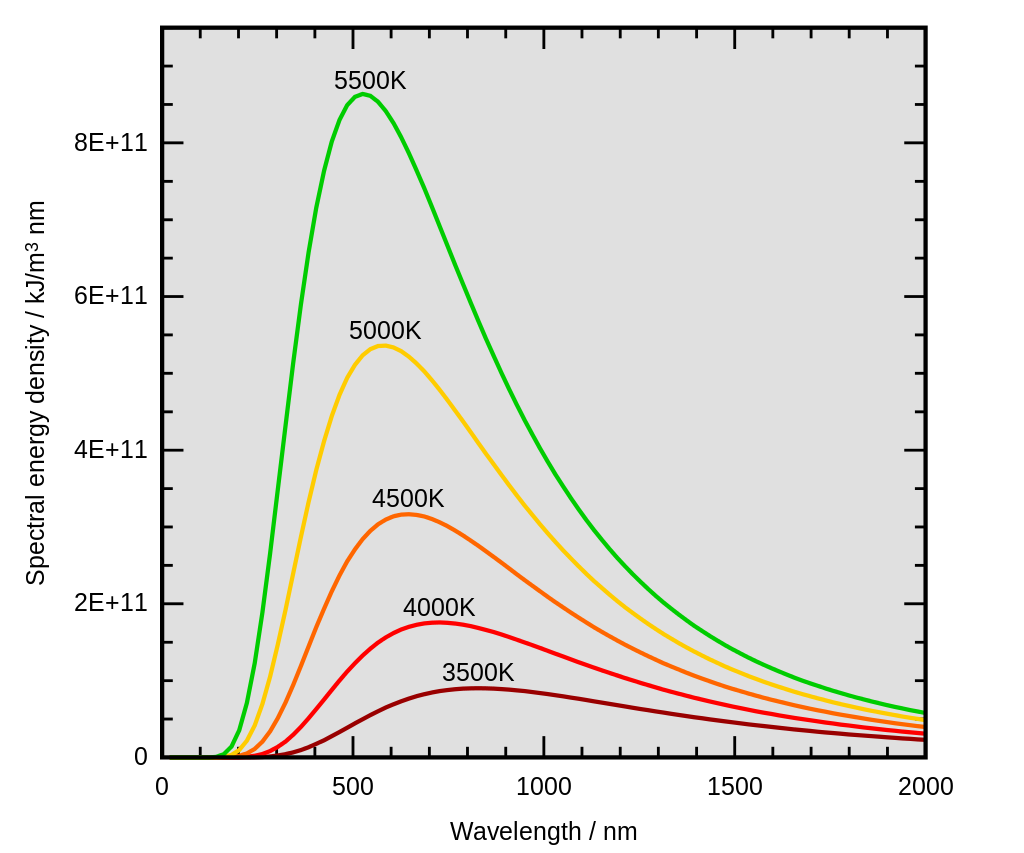
\includegraphics[width = 0.7\hsize]{./figures/radCorpoNero}
\caption{Radiazione emessa da un corpo nero a diverse temperature. \newline Si noti che, al crescere della temperatura la lunghezza d’onda corrispondente al massimo della curva si sposta verso valori più bassi.}
\label{fig:logo}
\end{figure}

\section{Catastrofe ultravioletta}
\par{Per studiare l’emissione di radiazioni delle pareti del corpo nero si è partiti dalle equazioni di Maxwell. Come risultato si erano ottenuti degli spettri che invece di scendere a zero per piccole lunghezze d’onda crescono indefinitamente. Si tratta della legge di \textit{Rayleigh-Jeans}.
Questa legge, come mostra la figura 2 è in netta contraddizione con i valori sperimentali.}

\begin{figure}[!h]
\centering
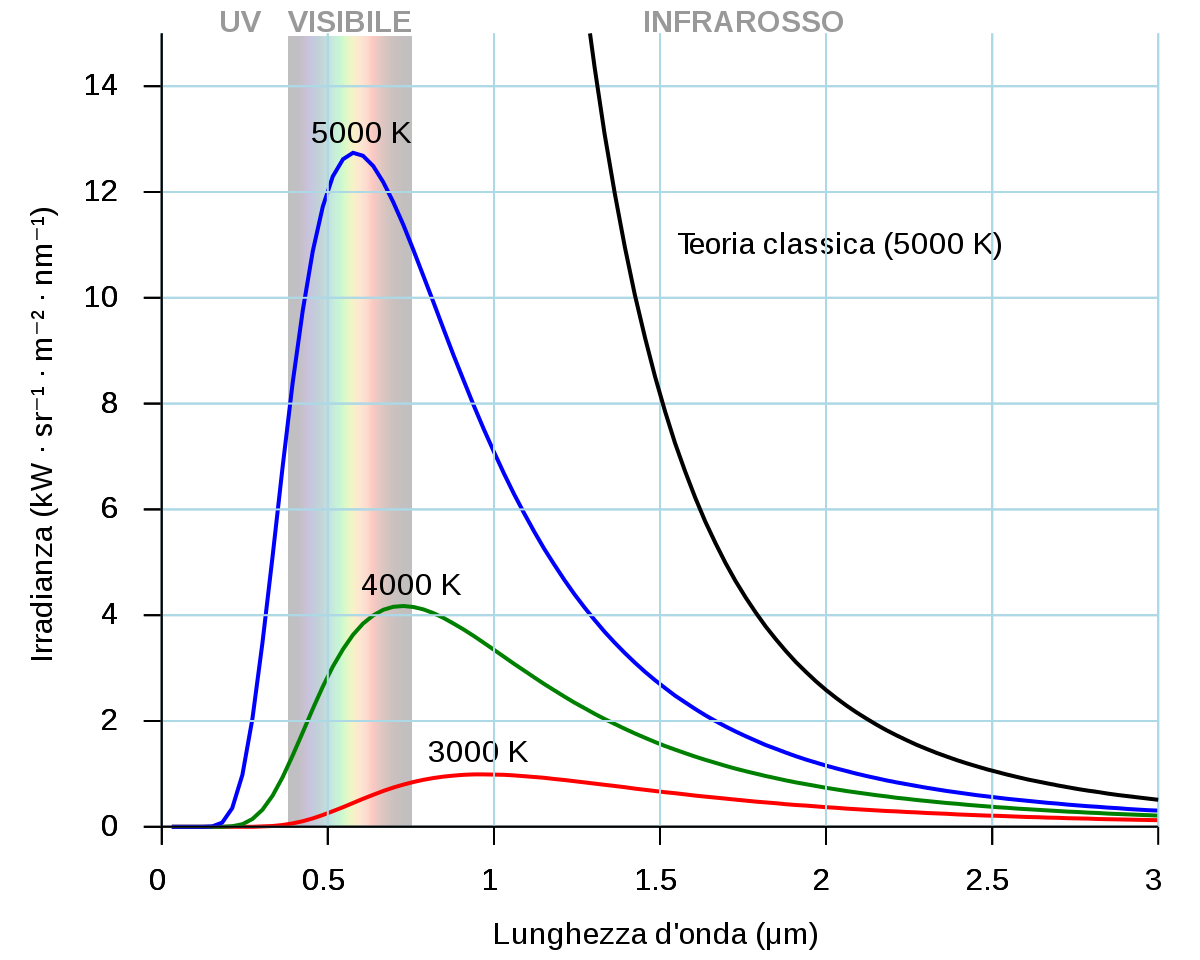
\includegraphics[width = 0.6\hsize]{./figures/catUltravioletta}
\caption{Discrepanza tra valori sperimentali e previsione teorica}
\label{fig:logo}
\end{figure}
\par{Ma c’è un’altra difficoltà: l’area della superficie compresa tra l’asse delle ascisse e la distribuzione spettrale $R(\lambda)$ fornisce l'irraggiamento totale.
$$ I(T) = \int_{0}^{\infty}{R(\lambda)d\lambda} $$
}
\par{La curva ottenuta sperimentalmente delimita una superficie finita, quindi non crea problemi. La legge di Rayleigh-Jeans non delimita una zona finita di piano, quindi in base a questa legge l’irraggiamento totale del corpo nero dovrebbe assumere un valore infinito.}
\par{Questo significa che il corpo nero emette un energia infinita; Evidente contraddizione del principio di conservazione dell’energia.
Questa palese dicrepanza tra dati sperimentali e teoria colpì talmente i fisici che fu definita \textit{catastrofe ultravioletta}.}

%\section{Integrali impropri}
%\par{Come accennato precedentemente nel par 1.3, è possibile determinare l’area sottesa alla curva $R(\lambda)$ tramite il calcolo infinitesimale. Ma come ci si comporta quando l’intervallo di integrazione è $[0; \infty)$ ?}
%\par{Nel caso in cui la funzione non sia continua nell’intervallo di integrazione, oppure almeno uno degli estremi di integrazione non sia finito si parla di integrale improprio}
%\par{Come accennato precedentemente nel par 1.3, è possibile determinare l’area sottesa alla curva $R(\lambda)$ tramite il calcolo infinitesimale. Ma come ci si comporta quando l’intervallo di integrazione è $[0; \infty)$ ? }
%\par{Nel caso in cui la funzione non sia continua nell’intervallo di integrazione, oppure almeno uno degli estremi di integrazione non sia finito si parla di integrale improprio.}
%\par{L’integrale improprio rappresenta l’estensione del concetto di integrale definito per funzioni che presentano un numero finito di discontinuità, oppure per funzioni il cui intervallo di integrazione risulta illimitato.}
%\par{Si dividono in integrali impropri di \textbf{primo}, \textbf{secondo} e \textbf{terzo tipo}. }


%Gli integrali impropri di \textbf{primo tipo} sono integrali che hanno uno o entrambi gli estremi di integrazione non finiti.
%$$
%\int_{a}^{\infty}f(x)dx    \;\;\;\;\;\;
%\int_{-\infty}^{a}f(x)dx    \;\;\;\;\;\; 
%\int_{-\infty}^{\infty}f(x)dx 
%$$
%\par{Per calcolare il valore di tali integrali si integra la funzione in un intervallo finito e poi si passa al limite facendo tendere all’infinito uno o entrambi gli estremi di integrazione: }
%$$
%\lim_{t\to\infty}\int_{a}^{t}f(x)dx \;\;\;\;\;\;
%\lim_{t\to-\infty}\int_{t}^{b}f(x)dx \;\;\;\;\;\;
%\lim_{(t,k)\to(\infty,-\infty)}\int_{k}^{t}f(x)dx \;\;\;\;\;\;
%$$
%\par{In base al valore ottenuto si possono distinguere 3 diversi} casi:
%\begin{itemize}
%\item Se il valore del limite è finito l'integrale improprio è convergente.
%\item Se il valore del limite è infinito l'integrale improprio è divergente.
%\item Se il valore del limite non esiste l'integrale improprio è indetermiato.
%\end{itemize}
%\par{Gli integrali impropri di \textbf{secondo tipo} hanno almeno un punto di %discontinuità nell'intervallo di integrazione}

%[To be continued]


\section{I Quanti di Planck}
\par{Il problema del corpo nero, già affrontato da numerosi fisici in precedenza, fu parzialmente risolto da \textit{Max Planck} nell'ottobre del 1900.}
\par{Fino ad allora si era supposto che gli atomi delle cavità interne del corpo nero scambiassero energia in modo continuo. Planck invece introdusse brillantemente una nuova ipotesi che permettesse di spiegare il fenomeno del corpo nero.}
\par{Gli scambi energetici tra gli atomi delle cavità interne e le radiazioni elettromagnetiche avvengono attraverso passaggi di  pacchetti di energia, o come li chiamò lo stesso Planck, \textit{}{quanti}.}
\par{Secondo lo scienziato tedesco l'energia $E$ scambiata tra atomi delle pareti è direttamente proporzionale alla frequenza $\nu$ dell'onda elettromagnetica assorbita o emessa secondo la formula: $$E = nh\nu$$ con $h$ un valore costante e $n$ è un intero positivo.}
\par{Il valore $h$ è detto  \textbf{Costante di Planck} e il suo valore è circa}
$$ h = \SI{6.62607e-34}{\joule\second}$$
\par{Per comprendere la teoria di Planck si può supporre che gli atomi del corpo nero si comportino come minuscoli oscillatori. In particolare che si comportino come una corda fissata ai due estremi e in vibrazione.}
\begin{figure}[h]
\centering
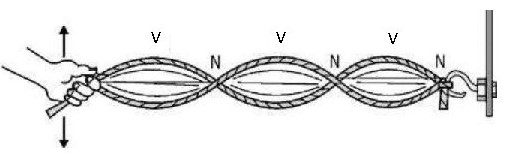
\includegraphics[width = 0.7\hsize]{./figures/ondaStaz}
\caption{Moto di un onda stazionaria \newline Si noti che alcuni punti sono sempre fermi, questi sono detti nodi.}
\label{fig:logo}
\end{figure}
\par{Una corda che si muove di moto stazionario non può oscillare a qualsiasi frequenza si voglia, ma può vibrare solo a determinate frequenze. Allo stesso modo gli atomi del corpo nero possono oscillare a determinate frequenze che sono discrete e fisse.}
\par{Un'onda elettromagnetica cede quindi la sua energia agli atomi di corpo nero, ma questi non sono in grado di oscillare a qualsiasi frequenza si voglia. Con questa ipotesi è possibile trovare un ottimo accordo tra la teoria modificata e i valori sperimentali.}
\par{La nuova previsione dell'irraggiamento di corpo nero di Planck tenendo conto dei quanti è la seguente:}
$$ R(\lambda,T) = \frac{2\pi c^2h}{\lambda^5}\frac{1}{e^{hc/\lambda kT}-1} $$
\par{Nonostante il successo del suo procedimento, egli credette per lungo tempo che la sua teoria fosse solo una sorta di strumento matematico, che non trovava ragion d’essere nei reali scambi di energia tra materia e radiazione. Egli non sospettava affatto che la meccanica classica e l’elettrodinamica potessero fallire. Si dice spesso che Planck abbia passato il resto della sua vita nel tentativo di rimuovere l’ipotesi della quantizzazione degli scambi energetici.}

%%%%%%%%%%%%%%%%%%%%%%%%%%%%%%%%%%%%
\chapter{Analisi dell'irraggiamento spettrale}
\section{Massimi, minimi e legge di Wien}
\par{Come abbiamo visto nella \texttt{figura 1.2} lo spettro di corpo nero ha dei \textit{picchi} che sono più o meno alti in funzione della temperatura.}
\par{Iniziamo con il definire matematicamente questi punti, che sono detti \textbf{massimi}.}

\begin{definition}
Data una funzione $y = f(x)$, definita in un intervallo $[a;b]$, il punto $x_0$ si dice \textbf{massimo relativo} se esiste un intorno $I_{x_0}$ di $x_0$ tale che $f(x_0)$ è maggiore o uguale al valore della funzione per ogni $x$ dell'intorno $I_{x_0}$.
In simboli: $$ f(x_0) \geq f(x) \; \forall x \in I_{x_0} $$
\end{definition}

\begin{figure}[!h]
\centering
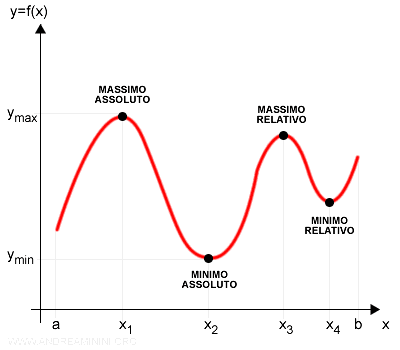
\includegraphics[width = 0.5\hsize]{./figures/maxmin}
\caption{Esempio di punti di massimi e minimi relativi e assoluti}
\label{fig:logo}
\end{figure}

In maniera analoga al massimo relativo possiamo definire il minimo relativo.

\begin{definition}
Data una funzione $y = f(x)$, definita in un intervallo $[a;b]$, il punto $x_0$ si dice \textbf{minimo relativo} se esiste un intorno $I_{x_0}$ di $x_0$ tale che $f(x_0)$ è minore o uguale al valore della funzione per ogni $x$ dell'intorno $I_{x_0}$. In simboli:
$$ f(x_0) \leq f(x) \; \forall x \in I_{x_0} $$
\end{definition}
\par{Massimi e minimi si dicono relativi perche sono in relazione all'intorno in cui sono definiti. I massimi e minimi assoluti invece sono i punti massimi e minimi che la funzione può assumere nell'intervallo in cui è definita.}

\begin{definition}
Data una funzione $y = f(x)$, definita in un intervallo $[a;b]$ si dice \textbf{massimo} (o \textbf{minimo}) \textbf{assoluto} della funzione il valore massimo (o minimo) tra i massimi (o minimi) relativi e i valori che la funzione assume agli estremi dell'intervallo.
\end{definition}
\par{Nel caso dell'irraggiamento $R(\lambda,T)$ esiste un solo punto di massimo relativo che quindi corrisponde al punto di massimo assoluto. Questo punto dipende esculivamente dalla temperatura del corpo nero. In particolare questi punti di massimo seguono una legge empirica nota come \textbf{legge dello spostamento di Wien}. }
$$ \lambda _{max} = b/T $$
\par{Dove $b = \SI{2.8977685e-3}{\meter\kelvin} $ \newline La lunghezza d'onda $\lambda _{max}$ per la quale è massima l'emissione radiattiva è quindi inversamente proporzionale alla temperatura $T$ alla quale è posto.}

\begin{figure}[!h]
\centering
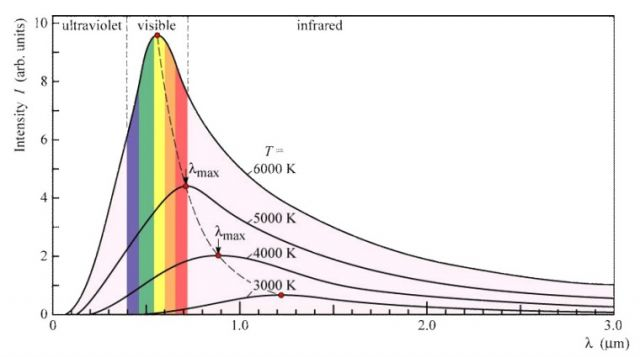
\includegraphics[width = 0.5\hsize]{./figures/leggeWien}
\caption{Legge dello spostamento di Wien}
\label{fig:logo}
\end{figure}

\par{La legge dello spostamento di Wien può essere utilizzata anche per determinare la temperatura di superficie di una stella conoscendo solo la lunghezza d'onda della radiazione emessa in maggioranza, ossia il colore con cui la stella ci appare.}
\par{Ad esempio, per la stella \textit{Sirio} la lunghezza d'onda per la quale il valore di irraggiamento spettrale è massimo è $\SI{240}{\nano\meter}$, che corrisponde al colore bianco-azzurro. Di conseguenza la sua temperatura superficiale sarà
$$ T = \frac{\SI{2898}{\micro\meter \kelvin}}{\SI{240}{\nano\meter}} = \SI{12000}{\kelvin} $$}


%Ma non solo, questi \textit{picchi} si trovano anche in corrispondenza di una certa lunghezza d'onda $\lambda$ che dipende esclusivamente dalla temperatura.

\section{Integrali impropri e legge di Stefan-Boltzmann}

\par{Come accennato precedentemente nel \texttt{paragrafo 1.3}, è possibile determinare l’area sottesa alla curva $R(\lambda,T)$ tramite il calcolo infinitesimale. Il valore di questa superficie dimensionalmente è la potenza complessiva, emessa sotto forma di radiazioni dal corpo nero a una data temperatura, diviso la superficie di emissione. Per calcolare il valore di questa superficie è necessario svolgere un integrale improprio, dato che uno degli estremi di integrazione è $+\infty$.}
\par{Inanzi tutto riscriviamo $R$ in funzione della frequenza $\nu$ anziche della lunghezza d'onda $\lambda$. }
$$ \int_{0}^{+\infty}R(\lambda,T)d\lambda = \int_{0}^{+\infty}{R(\nu,T)}d\nu $$
$$ \int_{0}^{+\infty}\frac{2\pi h\nu^3}{c^2}\frac{1}{e^{ \frac{h\nu}{kT} }-1}d\nu $$ 
\par{Procediamo riarrangiando l'integrale in funzione della variabile adimensionale 
$$t = \frac{h\nu}{kT}$$
in modo che $\nu \to 0 \Longrightarrow t \to 0 $ e $\nu \to +\infty \Longrightarrow t \to +\infty $.\newline Attuando la sostituzione si ha 
$$ \frac{2\pi k^4 T^4}{c^2 h^3}\int_{0}^{+\infty}\frac{t^3}{e^t-1}dt $$
Abbiamo ottenuto il prodotto tra una costante e un integrale improprio. Questo integrale è molto difficile da risolvere analiticamente, ma possiamo verificarne il valore tramite l'integrazione numerica.}
\par{Per farlo operiamo un cambio di variabile che riscali il dominio di integrazione da $t \in (0;+\infty)$ a $s \in (0;1)$. La sostituzione ad assicurarci questo è 
$$ s = \frac{t}{t+1} $$
Da questa adesso determiniamo sia $t$ sia il differenziale $dt$:
$$ t = \frac{s}{s-1} \;\;\;\;\;\; dt = \frac{ds}{(1-s)^2} $$
Da cui, operando il cambio di variabile nell'integrale
$$  \int_0^1 \frac{(\frac{s}{1-s})^3}{e^{\frac{s}{1-s}}-1}\frac{ds}{(1-s)^2} $$
$$ = \int_0^1 \frac{s^3}{(1-s)^5 (e^{\frac{s}{1-s}}-1)}ds $$
Adesso, con il supporto di un computer, possiamo determinare l'integrale con il \textbf{metodo dei trapezi}. Si suddivide l'intervallo di integrazione $(0, 1)$ in $1600$ parti uguali e si calcola l'area dei trapezi di base $1/1600$ e altezze date dal valore di f(x) agli estremi di ogni intervallo.
}
\begin{figure}[!h]
\centering
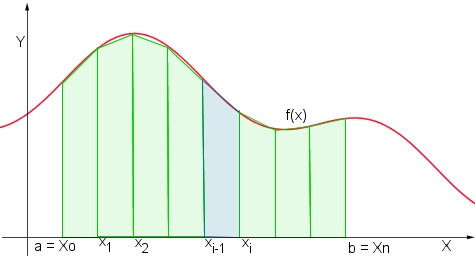
\includegraphics[width = 0.5\hsize]{./figures/metTrapezi}
\caption{Rappresentazione grafica del metodo dei trapezi}
\label{fig:logo}
\end{figure}
\par{Vediamo il codice sorgente scritto in C che ci permette di farlo.}
\lstinputlisting[language=C]{./sources/main.c}
%\lstlistoflistings
\par{L'integrazione numerica ci fornisce $6.49393940226683$, valore corretto fino alla \textit{dodicesima} cifra rispetto al valore di $\pi^4/15$}
\par{In conclusione}
$$ \int_0^{+\infty}R(\nu,T)d\nu = \frac{2\pi k^4T^4}{c^2h^3}\int_0^{+\infty}\frac{t^3}{e^t-1}dt = \frac{2\pi^5k^4}{15c^2h^3}T^4 $$
\par{Se denotiamo la costante che moltiplica $T^4$ con $\sigma$ si ha $$ I(T) = \sigma T^4 $$ Questa relazione è nota anche con il nome di \textbf{Legge di Stefan-Boltzmann}.}

%http://www.astro.unipd.it/progettoeducativo/UnitaDidattiche/UniDid_1.pdf
%http://profs.sci.univr.it/~zuccher/downloads/corpo-nero-EZ.pdf
%%%%%%%%%%%%%%%%%%%%%%%%%%%%%%%%%%%%
\chapter{Einstein e il fotone}
\section{Effetto fotoelettrico}
\par{Consideriamo adesso, dopo il corpo nero, un altro esempio in cui materia e radiazione interagiscono: l'\textit{effetto fotoelettrico}. E' proprio grazie all'analisi dell'effetto fotoelettrico che si poté dare una interpretazione fisica ai quanti di Planck.}
\par{Il fisico Philip Lenard scoprì già nel 1902 le leggi sperimentali dell'effetto, ma alcuni dettagli rimanevano inspiegati.}
\begin{figure}[!h]
\centering
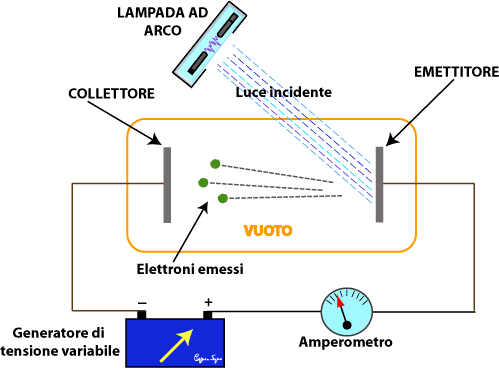
\includegraphics[width = 0.5\hsize]{./figures/effFoto}
\caption{Schematizzazione effetto fotoelettrico}
\label{fig:logo}
\end{figure}
\par{La \texttt{figura 3.1} schematizza un tipico apparato per studiare l'effetto. Una superficie di metallo, o emettitore, è investita da luce di frequenza $\nu$ e, se la frequenza è sufficietemente elevata, la luce provocherà l'emissione di elettroni dalla superficie. Stabilendo una differenza di potenziale appropriata tra l'emettitore e il collettore possiamo misurare una corrente elettrica.}

\begin{figure}[!h]
\centering
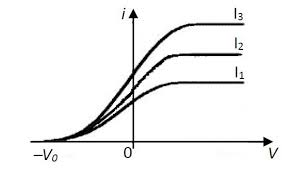
\includegraphics[width = 0.5\hsize]{./figures/potArr}
\caption{Grafico che riporta dati sperimentali misurati con l'apparecchio di \texttt{figura 3.1}}
\label{fig:logo}
\end{figure}

\par{La \texttt{figura 3.2} riporta la corrente elettrica $i$ in funzione della differenza di potenziale $V$ applicata. Se $V$ è positiva e abbastanza grande l'intensità di corrente raggiunge un valore masssimo. In questa situazione il collettore raccoglie \textit{tutti} gli elettroni emessi dall'emettitore.}
\par{Se riduciamo la differenza di potenziale a un numero negativo misureremo sempre una corrente fino a che ci sono elettroni che hanno energia cinetica maggiore del lavoro svolto dal campo elettrico. Tuttavia se continuiamo a ridurla raggiungiamo un valore $V_0$, detto potenziale di arresto a cui la corrente elettrica davvero si annulla. Questa differenza di potenziale moltiplicata per il valore della carica elettronica $e$ ci da il valore della energia cinetica $K_{max}$ dei fotoni emessi con massima energia:}
$$ K_{max} = e V_0 $$
\par{Il potenziale di arresto $V_0$ e quindi anche $K_{max}$ sono indipendenti dalla intensità luminosa incidente sull'emettitore. Nella \texttt{figura 3.2} per le tre curve l'intensità di luce era diversa, ma il potenziale di arresto rimane il solito.}

\begin{figure}[!h]
\centering
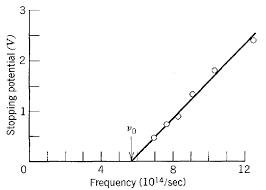
\includegraphics[width = 0.5\hsize]{./figures/stopPot}
\caption{Andamento del potenziale di arresto in funzione della frequenza}
\label{fig:logo}
\end{figure}
\par{Sperimentalmente possiamo notare che il potenziale di arresto varia in funzione della frequenza della radiazione incidente. Estrapolando la retta dai dati, in origine misurati da Millikan nel 1916 per una superficie di sodio, si nota che c'è una precisa frequenza di soglia $\nu_0$. Se la luce ha frequenza inferiore a questo valore l'effetto fotoelettrico cessa di manifestarsi e non viene emesso alcun elettrone.}


\section{Problematiche}
\par{Ci sono tre caratteristiche importanti dell'effetto fotoelettico che non possono essere spiegate nell'ambito della fisica classica ondulatoria della luce.}
\begin{enumerate}
\item \textit{Problema della intensità}.
\par{Secondo la teoria di Maxwell quando un onda elettromagnetica colpisce la superficie di un metallo, gli elettroni acquistano energia grazie al lavoro prodotto dal campo elettrico oscilante dell'onda. Aumentare l'intensità luminosa significa aumentare l'ampiezza di oscillazione del campo elettrico e quindi anche il lavoro svolto su ciascun elettrone. Ciò significa che l'energia cinetica degli elettroni debba aumentare quando la luce diventa più intensa. Ma la \texttt{figura 3.2} indica che $K_{max}$ è indipendente dalla intensità luminosa. }
\item \textit{Problema della frequenza}.
\par{Secondo la teoria classica l'effetto fotoelettrico dovrebbe poter avvenire per qualsiasi frequenza della luce a patto che essa sia abbastanza intensa da fornire l'energia necessaria per l'emissione di elettroni. Osservando la \texttt{figura 3.3} invece notiamo che esiste una frequenza di soglia $\nu_0$ al di sotto della quale l'effetto fotoelettrico non avviene per nessun livello di intensità della luce. }
\item \textit{Problema del ritardo}.
\par{L'energia luminosa nella teoria classica è distribuita in modo uniforme sul fronte d'onda. Quindi se la luce è abbastanza debole ci dovrebbe essere un intervallo di tempo misurabile tra il momento in cui la luce colpisce la superficie e quello dell'emissione degli elettroni. Durante questo intervallo gli elettroni assorbirebbero energia fino a che ne abbiano accumulata abbastanza per liberarsi. Tuttavia non è mai stato riscontrato alcun intervallo di tempo misurabile.}
\end{enumerate}

\section{Quantizzazione della luce di Einstein}
\par{Nel 1905 Einstein avanzo un ipotesi straordinaria. Suppose che in certe circostanze la luce si comporti come se la sua energia fosse concentrata in granuli, successivamente definiti \textit{fotoni}.}
\par{Un raggio di luce si comporta quindi come un flusso di particelle. Se nella teoria ondulatoria l'energia è uniformemente distribuita lungo il fronte d'onda, nell'ipotesi di Einstein l'energia è concentrate nelle particelle.}
\par{Secondo Einstain ogni fotone con una data frequenza $\nu$ trasposta un energia pari al prodotto della costante di Planck e la frequenza:}
$$ E = h\nu $$ 
\par{Se applichiamo l'ipotesi del fotone all'effetto fotoelettrico possiamo scrivere
$$ h\nu = W_e + K$$
In cui $h\nu$ è l'energia del fotone. Questa equazione ci dice che parte dell'energia del fotone viene assorbita dall'elettrone e impiegata come lavoro di estrazione $W_e$ e la restante parte si converte in energia cinetica $K$ dell'elettrone.}
\par{L'ipotesi di Einstein risolve le tre problematiche sollevate dalla teoria ondulatoria perché tutto l'effetto si riduce alla singola interazione fotone-elettrone.}
\par{Se aumentiamo l'intensità della luce aumentiamo il numero di fotoni e quindi il numero di elettroni che si separano dal metallo, ossia la corrente. Non varia invece l'energia cinetica massima degli elettroni. La prima obiezione è così risolta. }
\par{La seconda obiezione si risolve notando che per essere estratto l'elettrone deve interagire con un fotone con energia $h\nu$ maggiore del lavoro di estrazione $W_e$. Ciò significa che l'estrazione è possibile solo se la frequenza del fotone vale più di un certo valore $\nu_0$.}
\par{Anche il problema del ritardo è una conseguenza della teoria dei fotoni. L'energia è trasferita dalla luce all'elettrone sotto forma di blocchetto concentrato. Per questo motivo non si osserva alcun ritardo.}
\par{Quando Einstein propose la sua teoria dei fotoni i fenomeni di fotoelettricità non erano stabiliti sperimentalmente nel modo in cui li abbiamo oggi. Millikan fu il primo a sottoporre la teoria a rigide sperimentazioni di verifica. Anche se la teoria si mostrò in armonia con gli esperimenti Millikan rimase poco convinto che le particelle di luce potessero essere reali. Neppure Planck accettò immediatamente i fotoni. Fu invece proprio per i suoi studi sull'effetto fotoelettrico che Einstein ricevette il premio Nobel nel 1921.}
%%%%%%%%%%%%%%%%%%%%%%%%%%%%%%%%%%%%
\chapter{Gap in matematica}
\section{Discontinuità}
\par{L'energia trasportata dai fotoni, come abbiamo visto, non può assumere tutti i valori desiderati, ma solo un multiplo di $ h\nu$. Si può avere l'energia di due fotoni, tre fotoni, ma non ad esempio di due fotoni e mezzo. E' evidente che c'è un salto tra le due quantità. Un comportamento simile esiste anche in matematica e lo possiamo vedere nei punti di discontinuità.}

\begin{figure}[!h]
\centering
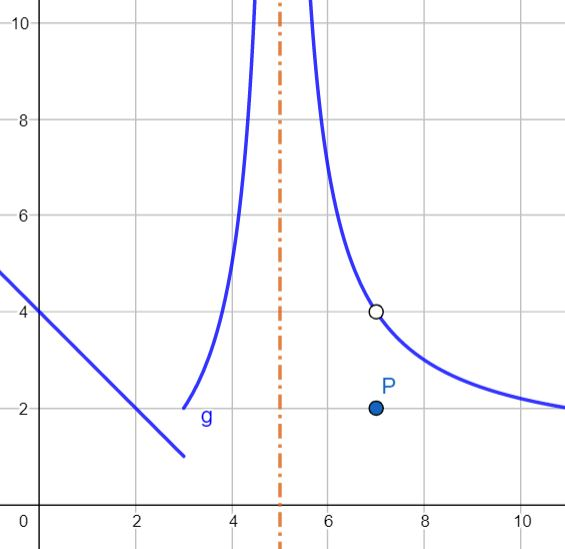
\includegraphics[width = 0.5\hsize]{./figures/disco}
\caption{Funzione contentente punti di discontinuià di prima, seconda e terza specie rispettivamente in x = 3, x = 5 e x = 7}
\label{fig:logo}
\end{figure}

\par{I punti di discontinuità sono di tre specie:}


\begin{definition}
Un punto $x_0$ si dice punto di discontinuità di prima specie per la funzione $f(x)$, quando per $x\to x_0$, il limite destro e il limite sinistro di $f(x)$ sono entrambi finiti ma diversi tra loro. 
$$ \lim_{x\to x_0^-}f(x) = l_1 \neq \lim_{x\to x_0^+}f(x) = l_2 $$
\end{definition}

\begin{definition}
Un punto $x_0$ si dice punto di discontinuità di seconda specie per la funzione $f(x)$, quando per $x\to x_0$, almeno uno dei due limiti, destro o sinistro, di $f(x)$ è infinito oppure non esiste. 
\end{definition}


\begin{definition}
Un punto $x_0$ si dice punto di discontinuità di terza specie per la funzione $f(x)$, quando esiste ed è finito il limite di $f(x)$ per $x \to x_0$ e $f(x_0)$ è diverso dal valore del limite.
\end{definition}





\section{Derivabilità}
\par{I punti di non derivabilità sono i punti in cui la funzione $f(x)$ è continua ma la derivata prima $f'(x)$ ha un punto di non continuità. I punti di non derivabilità sono di tre tipi.}
\begin{itemize}
    \item \textit{Flessi a tangente verticale}. Sono i punti $x_0$ in cui il limite per $x \to x_0$ di $f'(x)$ è $\pm \infty$. Si tratta di un punto di discontinuità di seconda specie.
    \item \textit{Cuspidi}. Sono i punti in cui per $x \to x_0$  il limite destro $f'_+(x) \to +\infty$ e il limite sinistro $f'_-(x) \to -\infty$, o viceversa. Si tratta di un punto di discontinuità di seconda specie.
    \item \textit{Punti angolosi}. Sono i punti in cui il limite della derivata prima $f'(x)$ per $x \to x_0$ destro e sinistro sono diversi tra loro e almeno uno dei due è finito. Si tratta quindi di un punto di discontinuità di prima specie se entrambi i limiti sono finiti, o di seconda specie se solo uno dei due è finito.
\end{itemize}

\begin{figure}[!h]
\centering
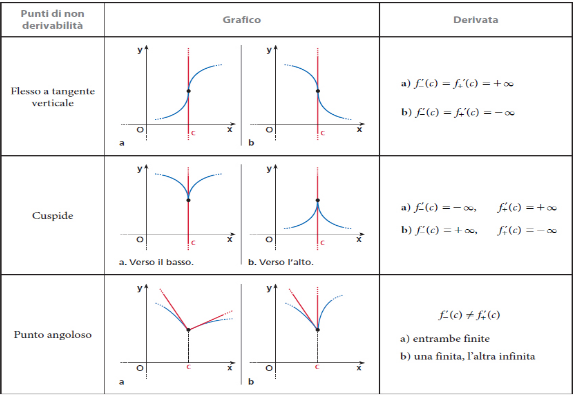
\includegraphics[width = 0.7\hsize]{./figures/nonder}
\caption{Esempi di punti di non derivabilità}
\label{fig:logo}
\end{figure}


%%%%%%%%%%%%%%%%%%%%%%%%%%%%%%%%%%%%
%\chapter{Conclusion}


%% bibliography
\nocite{*}
\bibliographystyle{abbrvnat}
\bibliography{sample}







\end{document}
